%--------------------------------------------------------------------------------------------------
%
\chapter{Background}
%--------------------------------------------------------------------------------------------------

The central subjects in the thesis revolve around statistical approaches to finding structure in one, two or more sets of variates. We will
introduce two methods that find structure in a single set of variates: $k$-means clustering and Principal Component Analysis. We will then present
Canonical Correlation Analysis (CCA), a method for studying two sets of variates. We will also briefly cover kernel method extensions of the methods.


\section{$k$-means}\label{sec:kmeans}

The $k$-means algorithm is perhaps the most well-known and widely-used clustering algorithm. Here, we present its application
to compute cross-lingual similarities. The idea is based on concatenating the corpus matrices, running standard $k$-means clustering to obtain the matrix of centroids, ``reversing" the concatenation step to obtain a set of aligned bases, which are finally used to compute cross-lingual similarities. See Figure~\ref{fig:kmeans} for overview of the procedure. The left side of Figure~\ref{fig:kmeans} illustrates the decomposition and the right side summarizes the coordinate change.

\section{Cross-Lingual Latent Semantic Indexing}\label{sec:LSI}

The second approach we consider is Cross-Lingual Latent Semantic Indexing (CL-LSI)~\cite{cl_lsi} which is a variant of LSI~\cite{lsi} for more than one language. The approach is very similar to $k$-means, where we first concatenate the corpus matrices, compute a decomposition, which in case of CL-LSI is a truncated Singular Value Decomposition (SVD), decouple the
 column space matrix and use the blocks to compute linear maps to a common vector space, where standard cosine similarity is used to compare documents.

 The method is based on computing a truncated singular value decomposition of the concatenated corpus matrix $X \approx U S V^T$. See Figure~\ref{fig:lsi} for the decomposition. Representing documents in ``topic`` coordinates is done in the same way as in the $k$-means case (see Figure~\ref{fig:kmeans}), we will describe how to compute the coordinate change functions.

\begin{figure}[tbp]
\centering
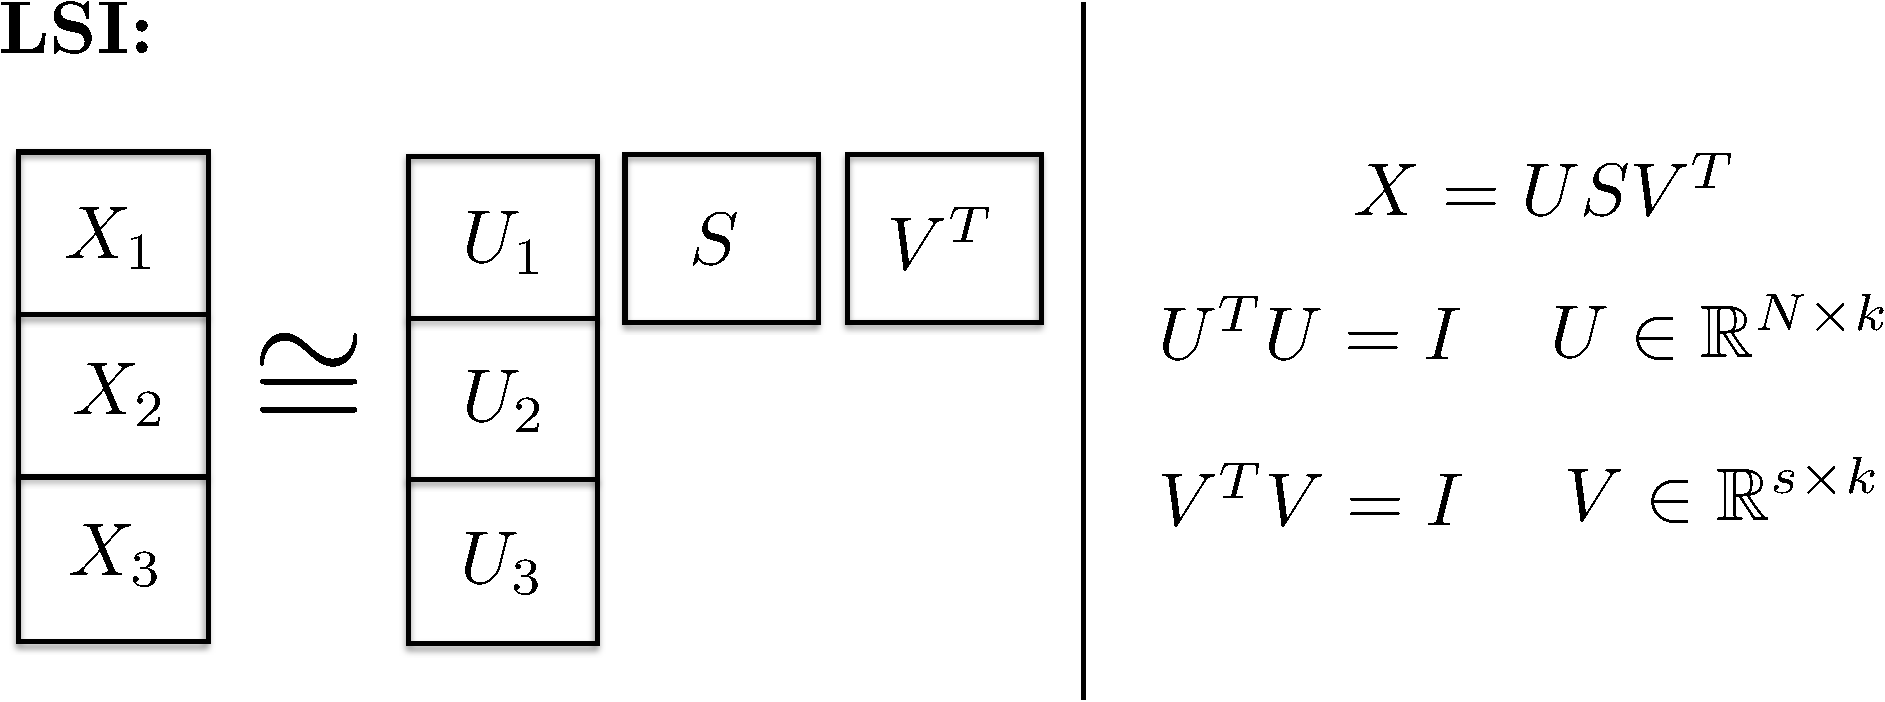
\includegraphics[width=10cm]{figures/lsi.pdf}
\caption{\label{fig:lsi} LSI multilingual corpus matrix decomposition.}
\end{figure}

The cross-lingual similarity functions are based on a rank-$k$ truncated SVD: $X \approx U \Sigma V^T,$ where $U \in \RR^{N \times k}$ are basis vectors of interest and $\Sigma \in \RR^{k \times k}$ is a truncated diagonal matrix of singular eigenvalues. An aligned basis is obtained by first splitting $U$ vertically according to the number of dimensions of each language: $U = [U_1^T \cdots U_m^T]^T$. Then, the same as with $k$-means clustering, we compute the pseudoinverses $P_i = (U_i^T U_i)^{-1} U_i^T$. The matrices $P_i$ are used to change the basis from the standard basis in $\RR^{n_i}$ to the basis spanned by the columns of $U_i$.

\paragraph{Implementation note}

  Since the matrix $X$ can be large we could use an iterative method like the Lanczos algorithm with reorthogonalization~\cite{golub} to find the left singular vectors (columns of $U$) corresponding to the largest singular values. It turns out that the Lanczos method converges slowly as the gap between the leading singular values is small. Moreover, the Lanczos method is hard to parallelize. Instead, we use a randomized version of the SVD~\cite{tropp} that can be viewed as a block Lanczos method. That enables us to use parallelization and speeds up the computation considerably.

To compute the matrices $P_i$ we used the QR algorithm~\cite{golub} to factorize $U_i$ as $U_i = Q_i R_i$, where $Q_i^TQ_i = I$ and $R_i$ is a triangular matrix. $P_i$ is then obtained by solving $R_i P_i = Q_i$.


\section{Canonical Correlation Analysis}

Canonical Correlation Analysis (CCA) ~\cite{Hotelling} is a general procedure for studying relationships between two sets of random variables. It is based on analyzing the cross-covariance matrix between two random vectors with the aim of identifying linear relationships between them. We will start with intuitions and then give a formal presentation.

Roughly speaking, given two random vectors $\mathcal{X}$ and $\mathcal{Y}$ we are interested in "non-trivial" pairs of functions $(f,g)$ such that there is a "dependence" between $f(\mathcal{X})$ and $g(\mathcal{Y})$. The "dependence" we consider is linear (possibly in a Hilbert space). The "non-triviality" of the functions is a requirement that guards us against trivial solutions, such as $f(x) := 0 \cdot x$, $g(y) := 0 \cdot y$ - that is, $f(\mathcal{X})$ and $\mathcal{X}$ should share some information, and analogously for $g(\mathcal{Y})$ and $\mathcal{Y}$. In other words, $f$ and $g$ should not destroy the original signals. When we are interested in more than one good pair of functions, for instance, a family of pairs $(f_i,g_i)$, we typically require additional constraints to prevent non-trivial solutions by enforcing that $f_i\left(\mathcal{X}\right)$ and $f_{j \neq i}\left(\mathcal{X}\right)$ share no information, and similarly for $g_i$. We are interested in essentially different function pairs.

There are several possible applications of such an analysis. For example, a common scenario involves analyzing objects $o \in \mathcal{O}$, where $\mathcal{O}$ is some underlying space, which are not directly observable, but are only observable as images of transformations $F: \mathcal{O} \rightarrow \RR^p$ and $G: \mathcal{O} \rightarrow \RR^q$. That is, we do not have access to $o$ but only to $\left(F(o), G(o)\right)$. Then finding function pairs $(f_i, g_i)$ so that $f_i(F(o))$ behave similarly as $g_i(G(o))$ can be interpreted as finding coupled parametrizations of image spaces of $F$ and $G$ which agree on $\mathcal{O}$. This enables applications such as cross-modal information retrieval, classification, clustering, etc. If $F$ encodes a visual image and $G$ encodes a textual description of the scene, we can perform text input based search over a collection of images, see~\cite{HardoonSS04}. Bi-lingual document analysis is another application, see~\cite{mrpqr}. The pattern functions $(f_i, g_i)$ themselves can be interesting to study for exploratory purposes.

Formally, let
$$ S = \{ \left( F(o_1), G(o_1) \right), \ldots, \left( F(o_n), G(o_n) \right) \} $$
represent a sample of $n$ pairs drawn independently at random according to the underlying distribution, where $F(x_i) \in \RR^p$ and $G(x_i) \in \RR^q$ represent feature vectors from $p$ and $q$-dimensional vector spaces. Let $X=[F(o_1), \ldots, F(o_n)]$ and let $Y=[G(o_1), \ldots ,G(o_n)]$ be the matrices with observation vectors as columns (using MATLAB notation).

The idea is to find two linear functionals (row vectors) $\alpha \in \RR^p$ and $\beta \in \RR^q$ so that the random variables $\alpha \cdot \mathcal{X}$ and $\beta \cdot \mathcal{Y}$ are maximally correlated ($\alpha$ and $\beta$ map the random vectors to random variables, by computing weighted sums of vector components). By using the sample matrix notation $X$ and $Y$ this problem can be formulated as the following optimization problem:

\begin{equation*}
\begin{aligned}
& \underset{\alpha \in \RR^{p}, \beta \in \RR^{q}}{\text{maximize}}
& & \frac{\alpha C_{XY} \beta'}{\sqrt{\alpha C_{XX} \alpha'} \sqrt{\beta C_{YY} \beta'}},
\end{aligned}
\end{equation*}
where $C_{XX}$ and $C_{YY}$ are empirical estimates of variances of $\mathcal{X}$ and $\mathcal{Y}$ respectively and $C_{XY}$ is an estimate for the covariance matrix. Assuming that the observation vectors are centered, the matrices are computed in the following way: $C_{XX} = \frac{1}{n-1}X X'$, $C_{YY} = \frac{1}{n-1}Y Y'$ and $C_{XY} = \frac{1}{n-1}X Y'$.
The optimization problem can be reduced to an eigenvalue problem and includes inverting the variance matrices $C_{XX}$ and $C_{YY}$. If the matrices are not invertible, one can use a regularization technique by replacing $C_{XX}$ with $(1- \kappa)C_{XX} + \kappa I$, where $\kappa \in [0,1]$ is the regularization coefficient and $I$ is the identity matrix.
A single canonical variable is usually inadequate in representing the original random vector and typically one looks for $k$ projection pairs $(\alpha_1, \beta_1),\ldots,(\alpha_k, \beta_k)$, so that $\alpha_i$ and $\beta_i$ are highly correlated and $\alpha_i$ is uncorrelated with $\alpha_j$  for $j \neq i$ and analogously for $\beta$.

The problem can be reformulated as a symmetric eigenvalue problem and solved efficiently. In case the dimensions of the problem $p$ and $q$ are large and observation vectors are sparse, one can consider an iterative method, for example Lanczos algorithm~\cite{LAL}). Alternatively, if the number of observation vectors $n$ is not prohibitively large, one can reformulate the problem to its dual representation which can be combined with a "kernel trick"~\cite{FBMJ} to yield nonlinear version of CCA.

A single canonical variable is usually inadequate in representing the original random vector and typically one looks for $k$ projection pairs $(w_i^1, w_j^1),\ldots,(w_i^k, w_j^k)$, so that $(w_i^{u})^T \mathcal{X}_i$ and $(w_j^{u})^T \mathcal{X}_j$ are highly correlated and $(w_i^{u})^T \mathcal{X}_i$ is uncorrelated with $(w_i^{v})^T \mathcal{X}_i$  for $u \neq v$ and analogously for $w_j^u$ vectors.


\section{Kernels and KCCA}
